\chapter{Fazit}
\label{chap:Fazit}
Die Arbeit schließt mit einer Zusammenfassung der Inhalte ab, auf welche eine kritische Auseinandersetzung mit verschiedenen Ergebnissen der Abschlussarbeit folgt und durch einen ausführlichen Blick auf mögliche Erweiterungen und weitere geleistete Arbeiten komplettiert wird.
 
	\section{Zusammenfassung}
	\label{sec:Zusammenfassung}
	Zu Beginn der Arbeit wurde die zu bearbeitende Problemstellung erläutert, anschließend wurden die theoretischen Hintergründe, das Umfeld der Problemstellung und die Datensätze vorgestellt. Der Hauptteil der Arbeit beschäftigt sich mit aufeinander aufbauenden Ansätzen des Transferlernens. Im ersten Schritt wurde gezeigt, dass ein Ansatz, ausgehend von einer nicht fokussierten Repräsentation fehlschlägt. Darauf folgend wurde ein Multi-Task-Ansatz zum gleichzeitigen Fokussieren und Lösen einer Regressionsaufgabe vorgestellt und evaluiert. Insbesondere die gefundene Repräsentation hat dabei deutlich die aktuelle Domäne widergespiegelt. Darauf aufbauend wurde ein Ansatz des modellbasierten Transferlernen vorgestellt. Die Ergebnisse erreichen eine ähnliche Leistung wie ein Modell, welches von einem Experten erstellt wurde. Zur \ac{hpo} der Aufgaben-Gewichtungsparameter wurde eine \ac{automl}-Erweiterung eingesetzt. Dabei hat sich gezeigt, dass der Hyperparameter einen deutlichen Einfluss auf das Ergebnis hat und die automatische Suche hilfreich ist. Abschließend wurde gezeigt, dass die Transfer-Lösung insbesondere für geringe Datenmengen gute Ergebnisse liefern kann. Begleitend zu der Vorstellung der Ansätze wurde jeweils eine Python-Implementierung des Ansatzes vorgestellt. 
			
	\section{Kritische Reflexion}
	\label{sec:KritischeReflexion}
	
	andere Domäne testen Greifer ist sehr klar		
	Daten	
				
	\section{Ausblick und weitere Arbeiten}
	\label{sec:AusblickWeitereArbeiten}
	In diesem letzten Unterkapitel werden weitere (vorläufige) Ergebnisse dargestellt und da die untersuchten Methoden 
	

	\subsection{Transfer auf Greiferdatensatz}
	\label{subsec:TransferGreiferDatensatz}
 	Die Annotationskosten sind je nach Art von Annotation und Aufwand unterschiedlich. Eine einfache Zuordnung eines Bildes zu einer, von zwei Klassen liegt dabei im einstelligen Cent-Bereich. Die Markierung eines Objektes in einem Bild mittels Rahmen verursacht Kosten im zweistelligen Cent-Bereich und die Markierung von Winkeln in einem Bild kann mehr als einen Euro kosten. 		

	\todo{Ergebnisse Transfer Greifer}
	
	\subsection{Autocrane-Datensatz}
	\label{subsec:AutocraneDatensatz}	
	Im Rahmen der Arbeit wurde ein Datensatz erarbeitet und Projektpartnern zur Verfügung gestellt. Eine spätere Veröffentlichung des Datensatzes unter der Adresse psiori.com ist geplant. Der Datensatz soll zu allgemeinen akademischen und pädagogische Zwecken genutzt werden dürfen. Alternativ kann Zugang zu dem Datensatz über die E-Mail-Adresse info@psiori.com erfragt werden.

	\subsection{Multi-Task}
	\label{subsec:MehrfacheAufgaben}
	Multi-Task-Lernen beschränkt sich nicht auf zwei Aufgaben. Die gezeigte Lösung kann um weitere Aufgaben erweitert werden. In Abbildung \ref{img:AusblickMultiTaskAnsatz} ist der erweitere Ansatz schematisch abgebildet. Wie in den bisherigen Ansätzen werden ausgehend von der Code-Schicht weitere Aufgaben bearbeitet. Durch die weiteren Aufgaben wird die Gewichtung der einzelnen Aufgaben noch schwerer. In Experiment \ref{sec:AutoTransferSecondCriterionAutoenocder} \todo{ref prüfen} wurde gezeigt, dass BOHB bei der Gewichtung helfen kann. Dieser erweiterte Ansatz soll in einem Anschlussprojekt für die Praxistauglichkeit untersucht werden. Der Aufwand, das bisher entwickelte Python-Modul zu erweitern, wird sich dabei in Grenzen halten. Insbesondere müssen im Konstruktor Erweiterungen zum Erstellen der Modelle der weiteren Aufgaben getätigt werden. An anderen Stellen wie z. B. der Methode zum Trainieren des Gesamtmodells wird keine Erweiterung notwendig sein, da bereits mit Listen gearbeitet wird.
	\begin{figure}[h]
		\centering
		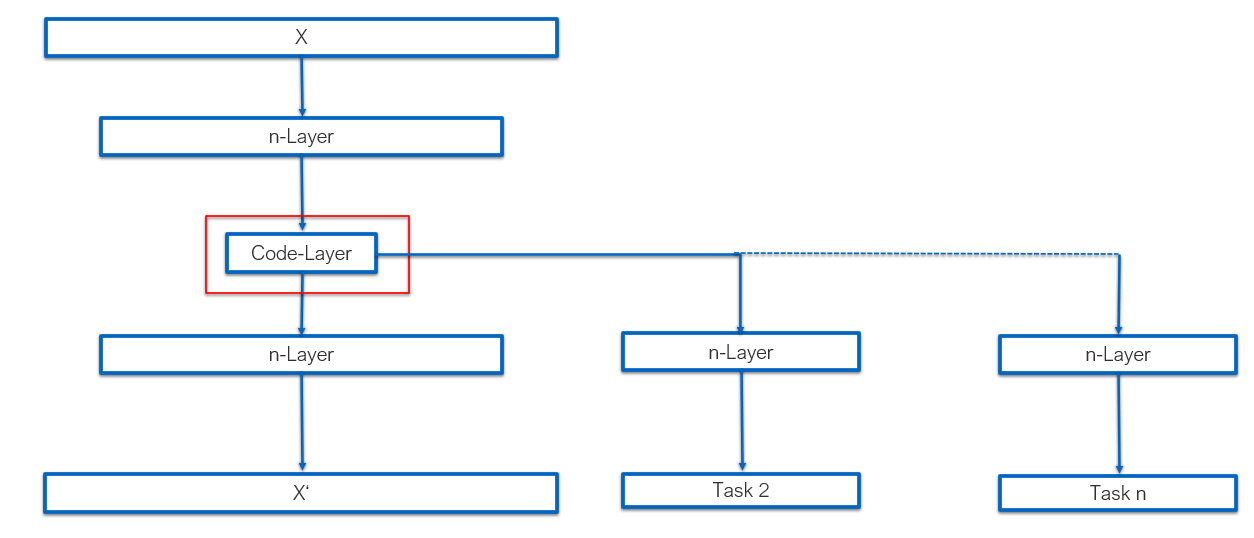
\includegraphics[width=0.5\textwidth, center]{bilder/FazitUndAusblick/MultiTaskAnsatz.PNG}
		\caption[Ausblick Multi-Task-Ansatz]{Multi-Task-Ansatz}
		\label{img:AusblickMultiTaskAnsatz}
	\end{figure}


	\subsection{Flexibilität der Werkzeuge}
	\label{subsec:FlexibilitätDerWerkzeuge}
	Die bisherigen Module sind starr bei der Anwendung. Es ist notwendig, ein Multi-Aufgaben-Modell zu erstellen, um anschließend den modellbasierten Transfer durchzuführen. Soll ein neuer modellbasierter Transfer durchgeführt werden, ist es zwingend erforderlich dies ausgehend des Multi-Aufgaben-Modells durchzuführen. Es ist nicht möglich einen modellbasierten Transfer, ausgehend von einem vorherigen Transfer durchzuführen. 
	Als mögliche Erweiterung der Module ist es empfehlenswert, eine Flexibilisierung des Gesamtansatzes durchzuführen. Durch eine Anpassung bei der Modellerstellung der Module, ist es möglich, dass die Abfolge nicht mehr notwendig ist. Es ist vorstellbar, dass ein neues Modell ausgehend von einer Architekturdefinition komplett neu trainiert wird, oder ausgehend von einem Autoencoder-Modell mit null bis beliebig vielen weiteren Aufgaben trainiert werden kann. Konkret muss im Konstruktor der Module eine Zusammenführung der bisher getrennten Ansätze durchgeführt werden.     
